closed loop stuff, explain

\begin{figure}[H]
  \centering
    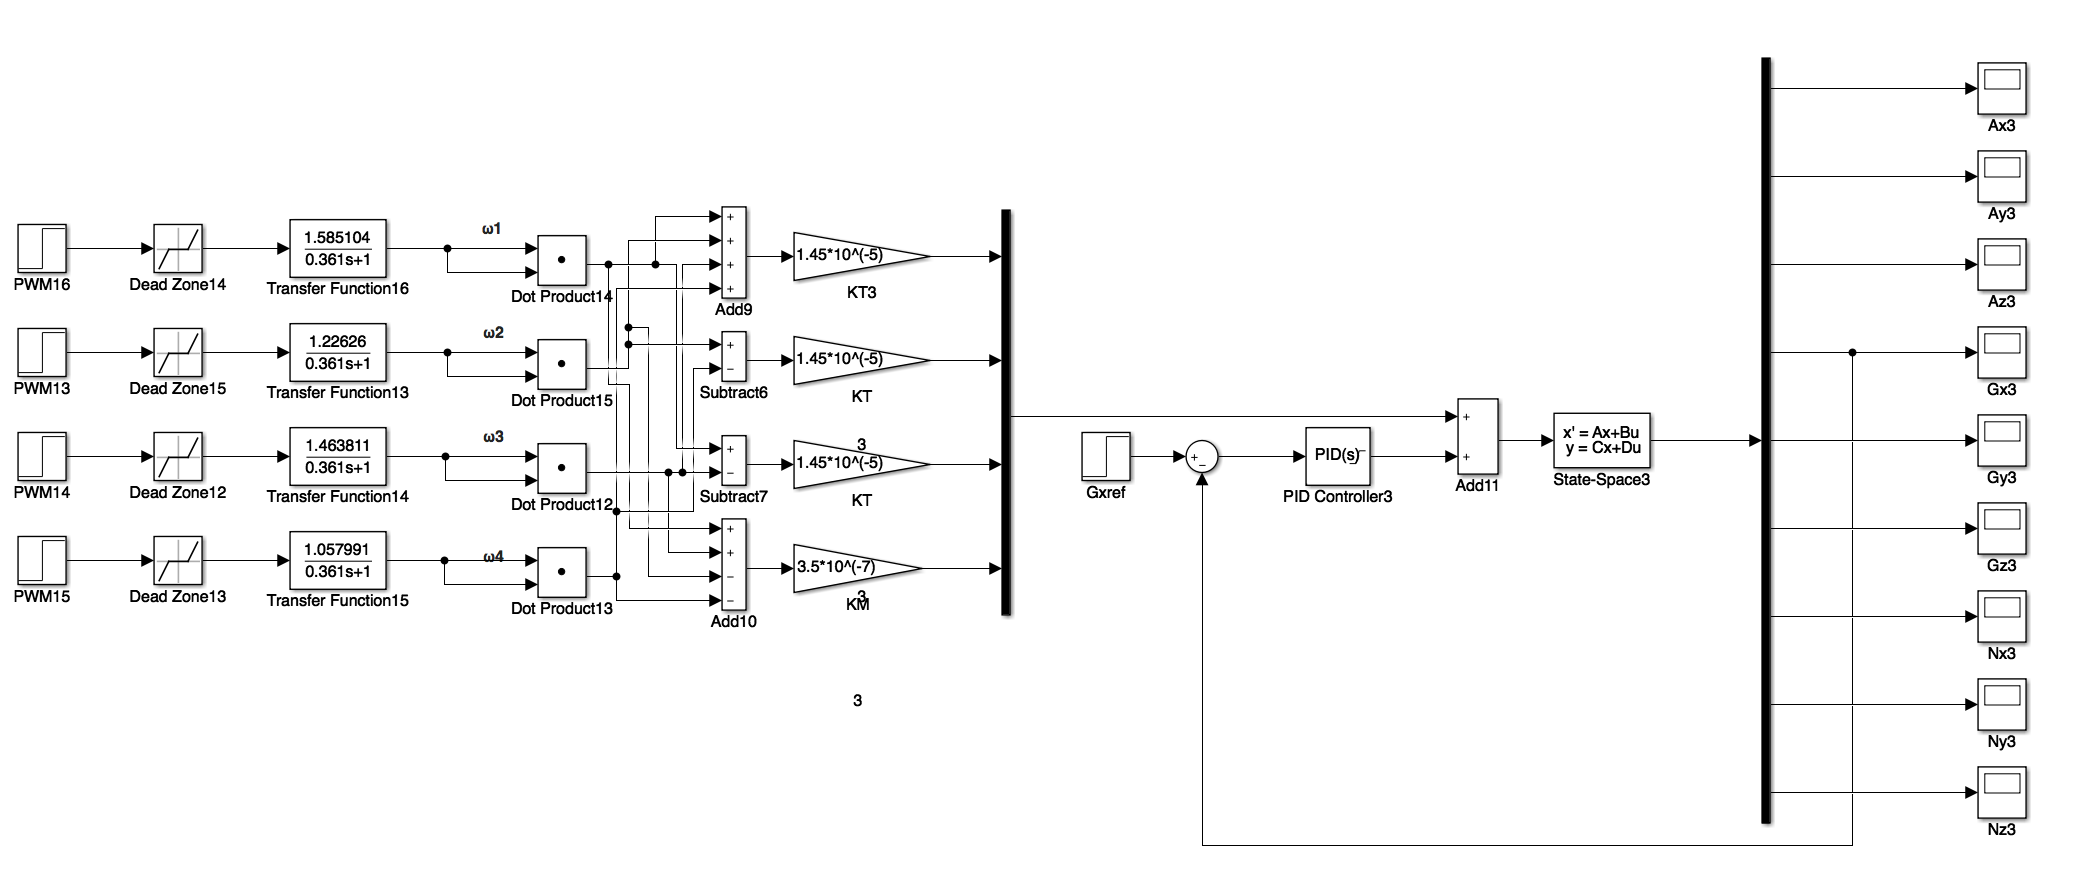
\includegraphics[width=1\textwidth]{images/closedloopGx.png}
	\caption{smth.}
	\label{closedloop1}
\end{figure}

using autotune, pid whatever stuff, maybe merge figures into one.

\begin{figure}[H]
  \centering
    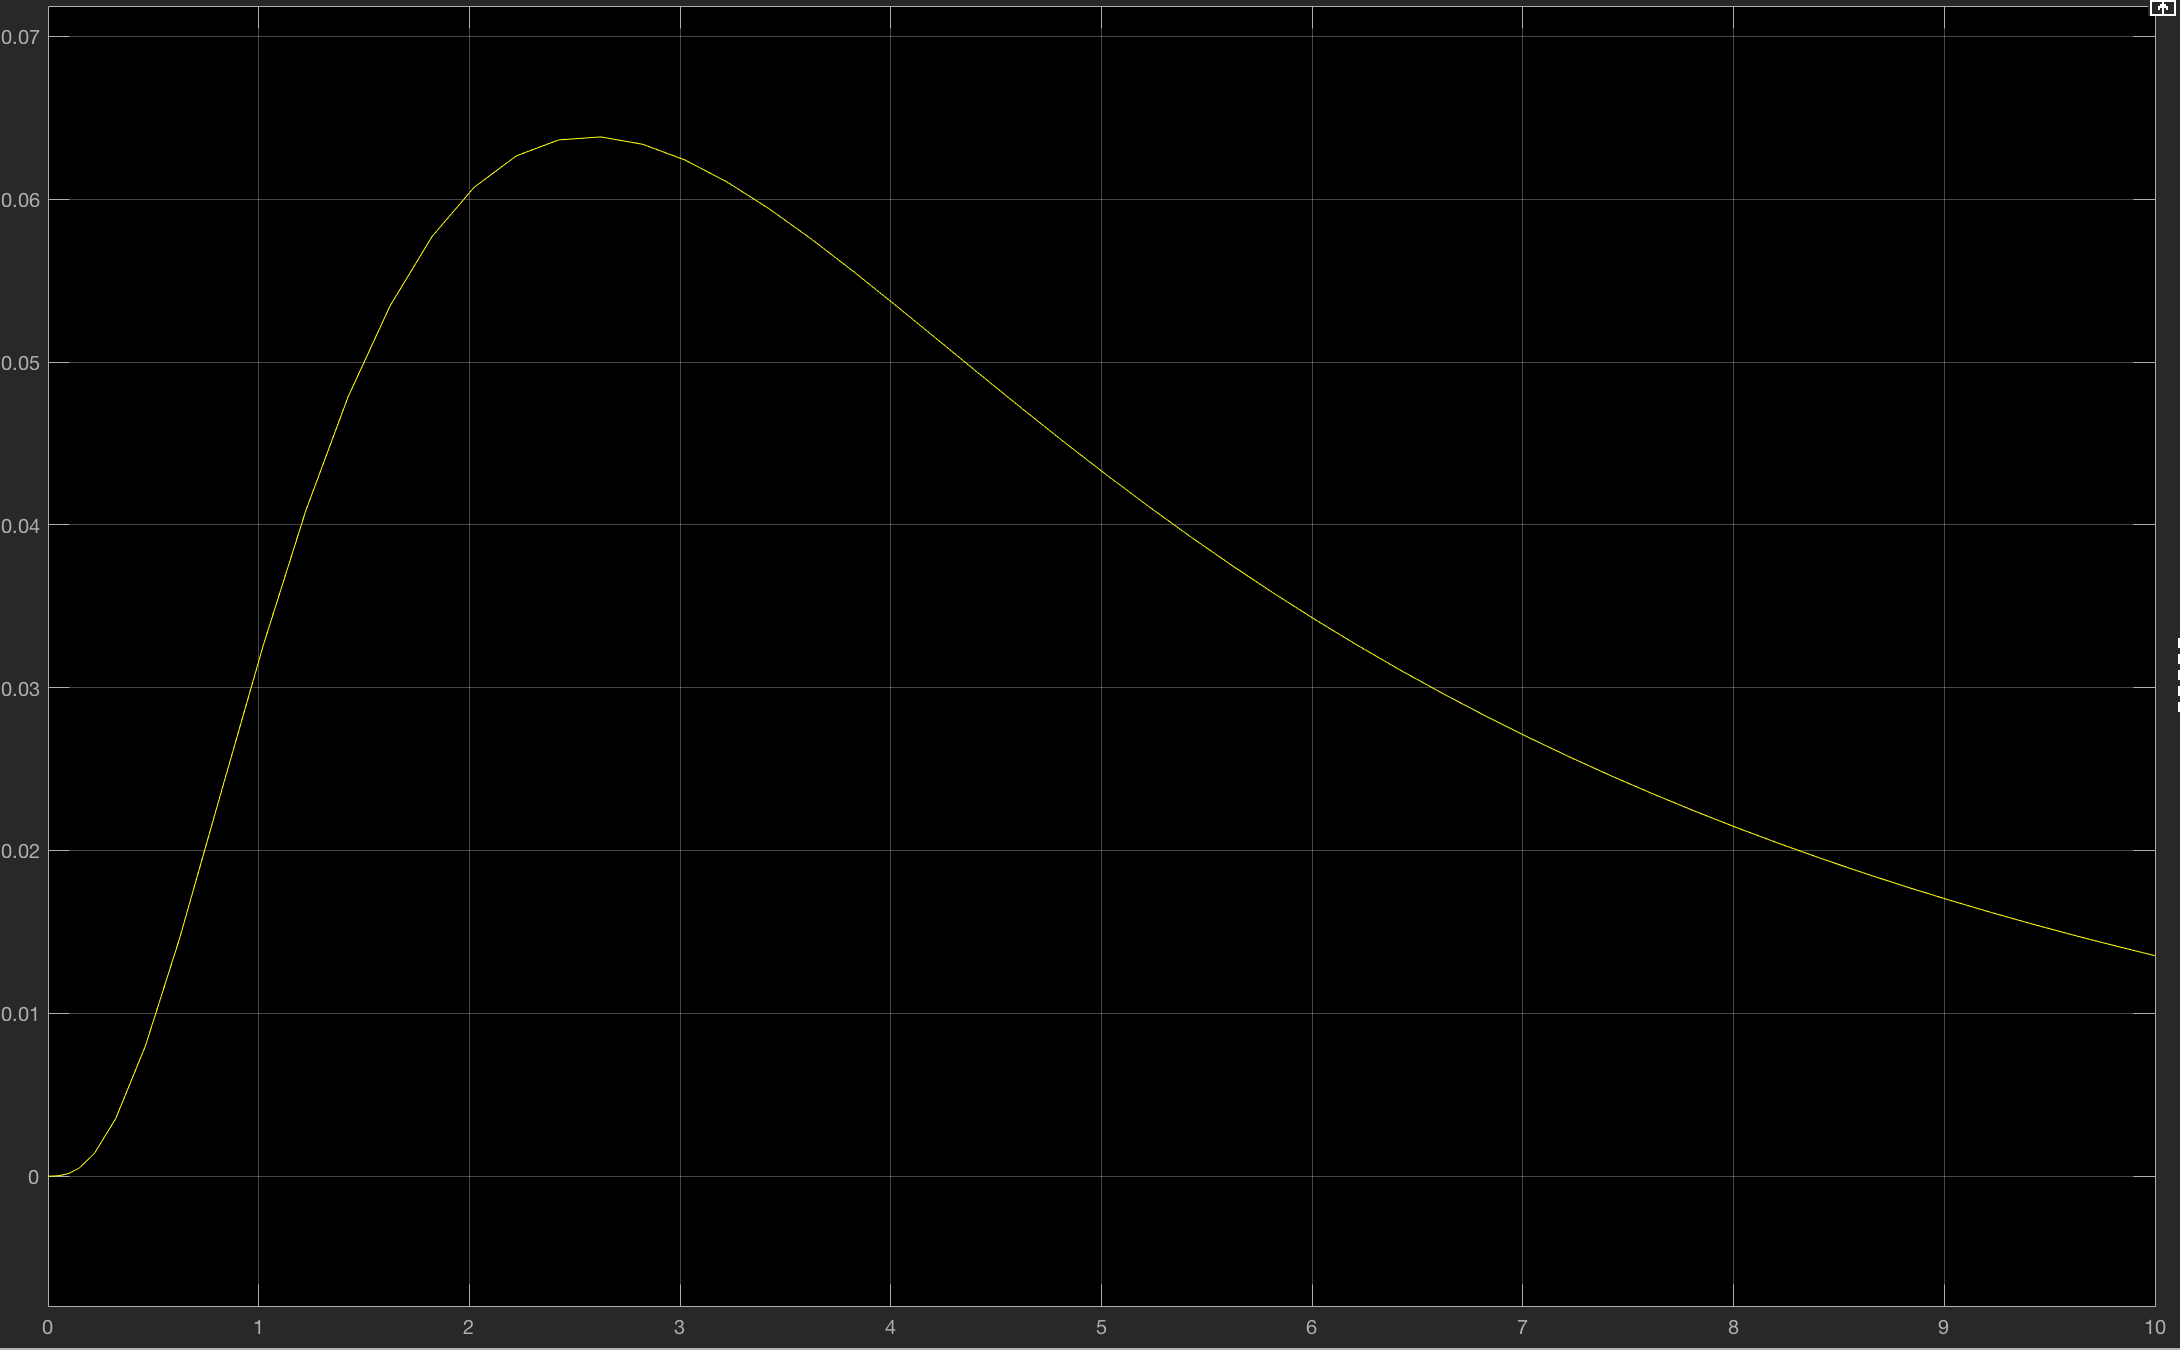
\includegraphics[width=1\textwidth]{images/closedloopGxstep.png}
	\caption{smth.}
	\label{closedloop2}
\end{figure}

\begin{figure}[H]
  \centering
    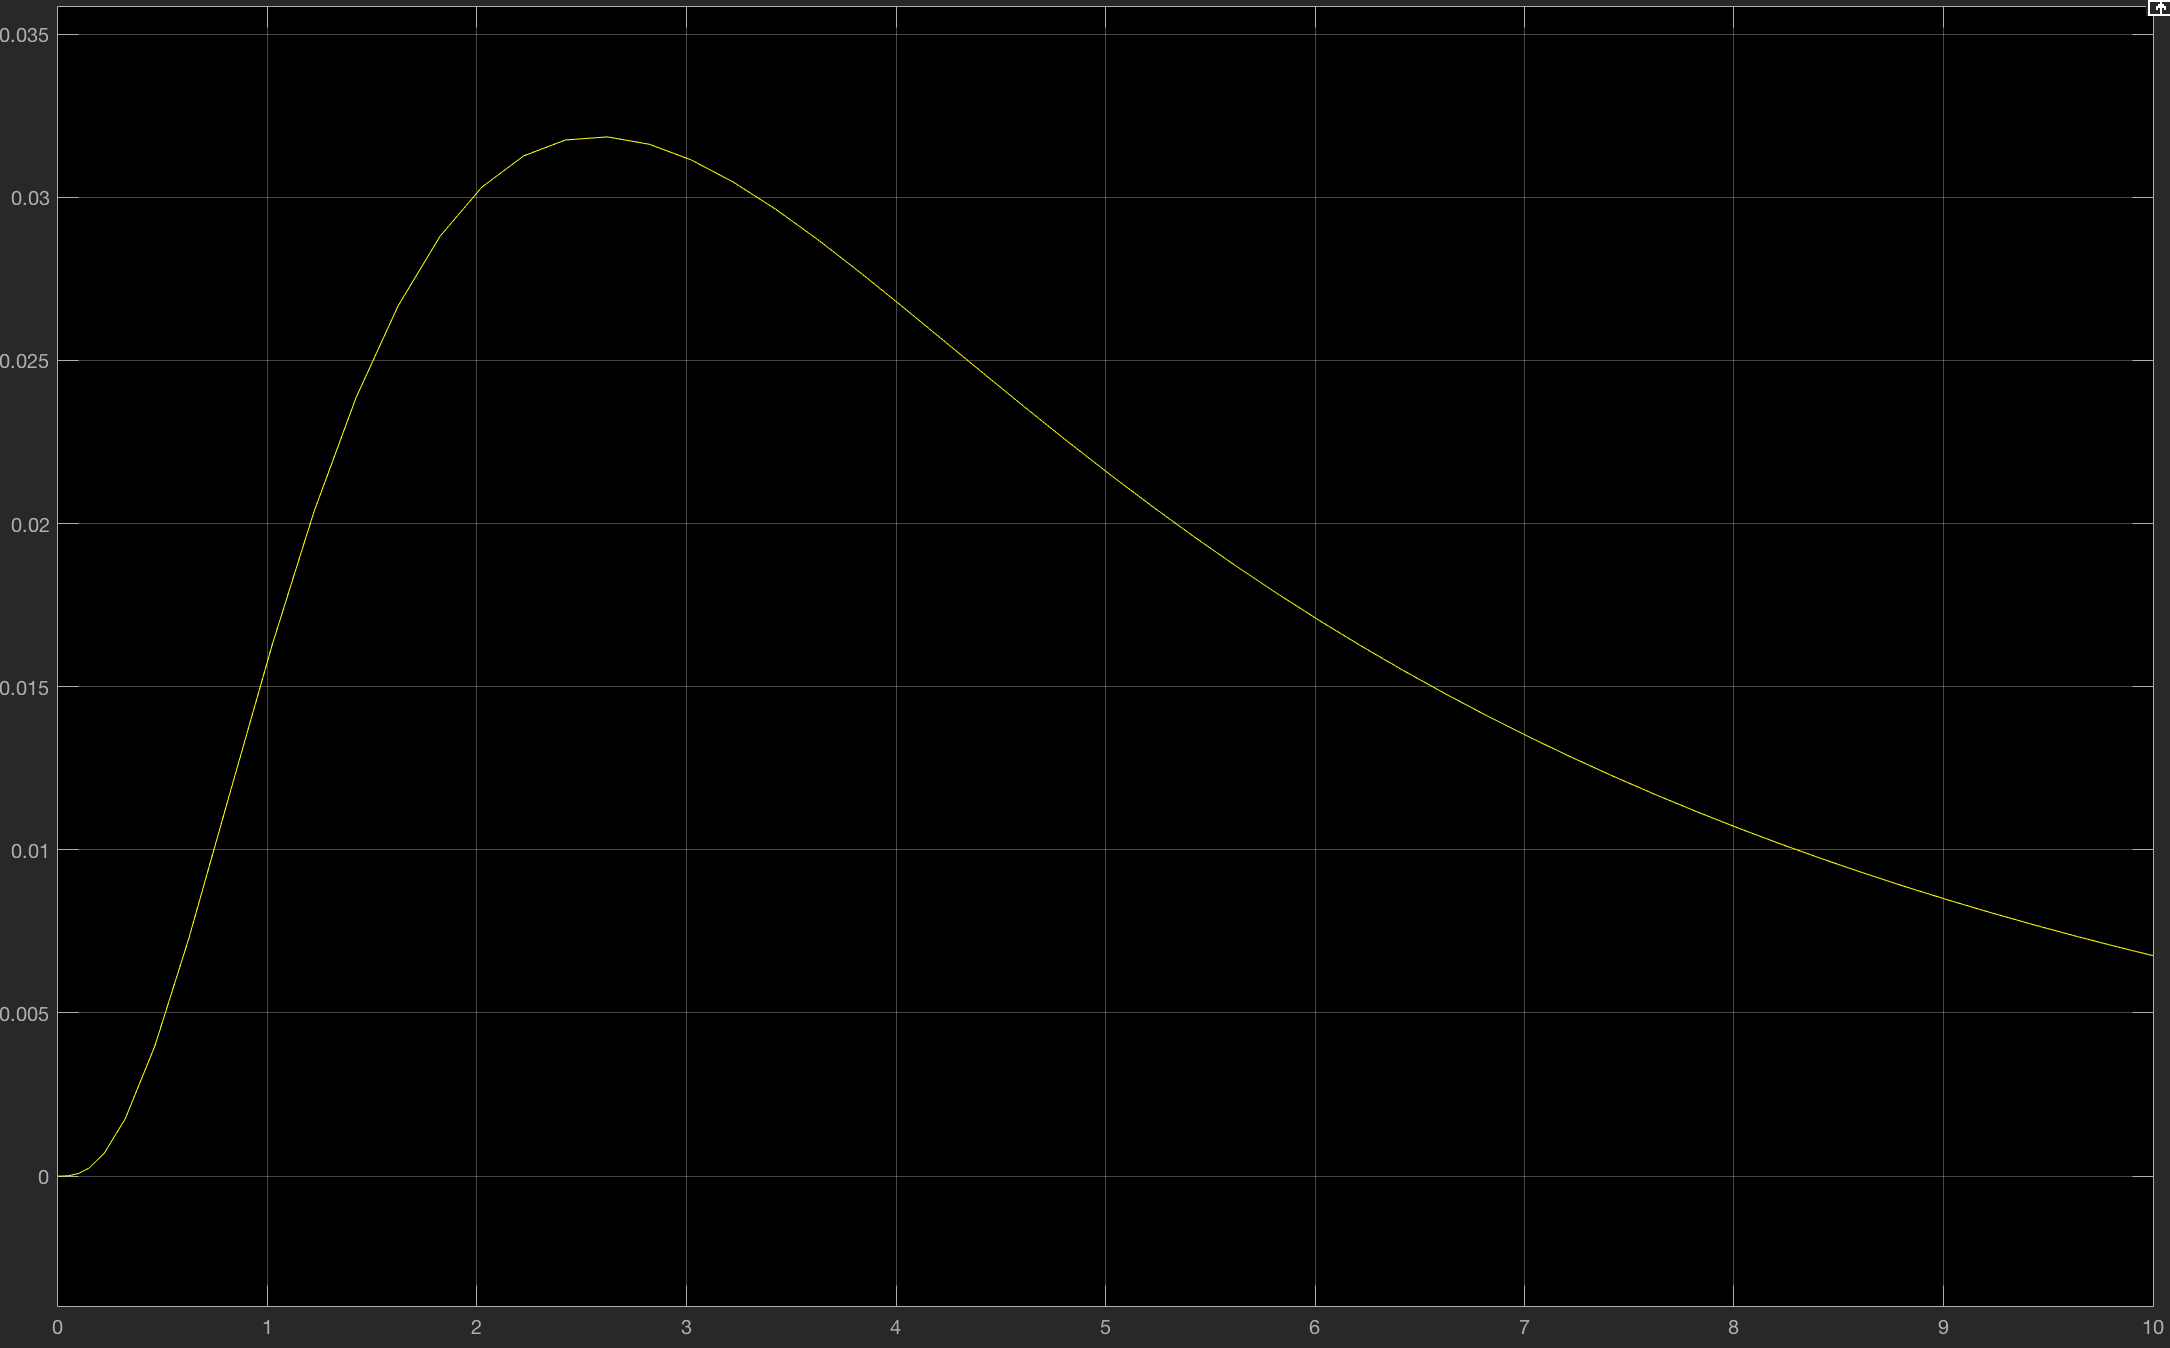
\includegraphics[width=1\textwidth]{images/closedloopGystep.png}
	\caption{smth.}
	\label{closedloop3}
\end{figure}

\begin{figure}[H]
  \centering
    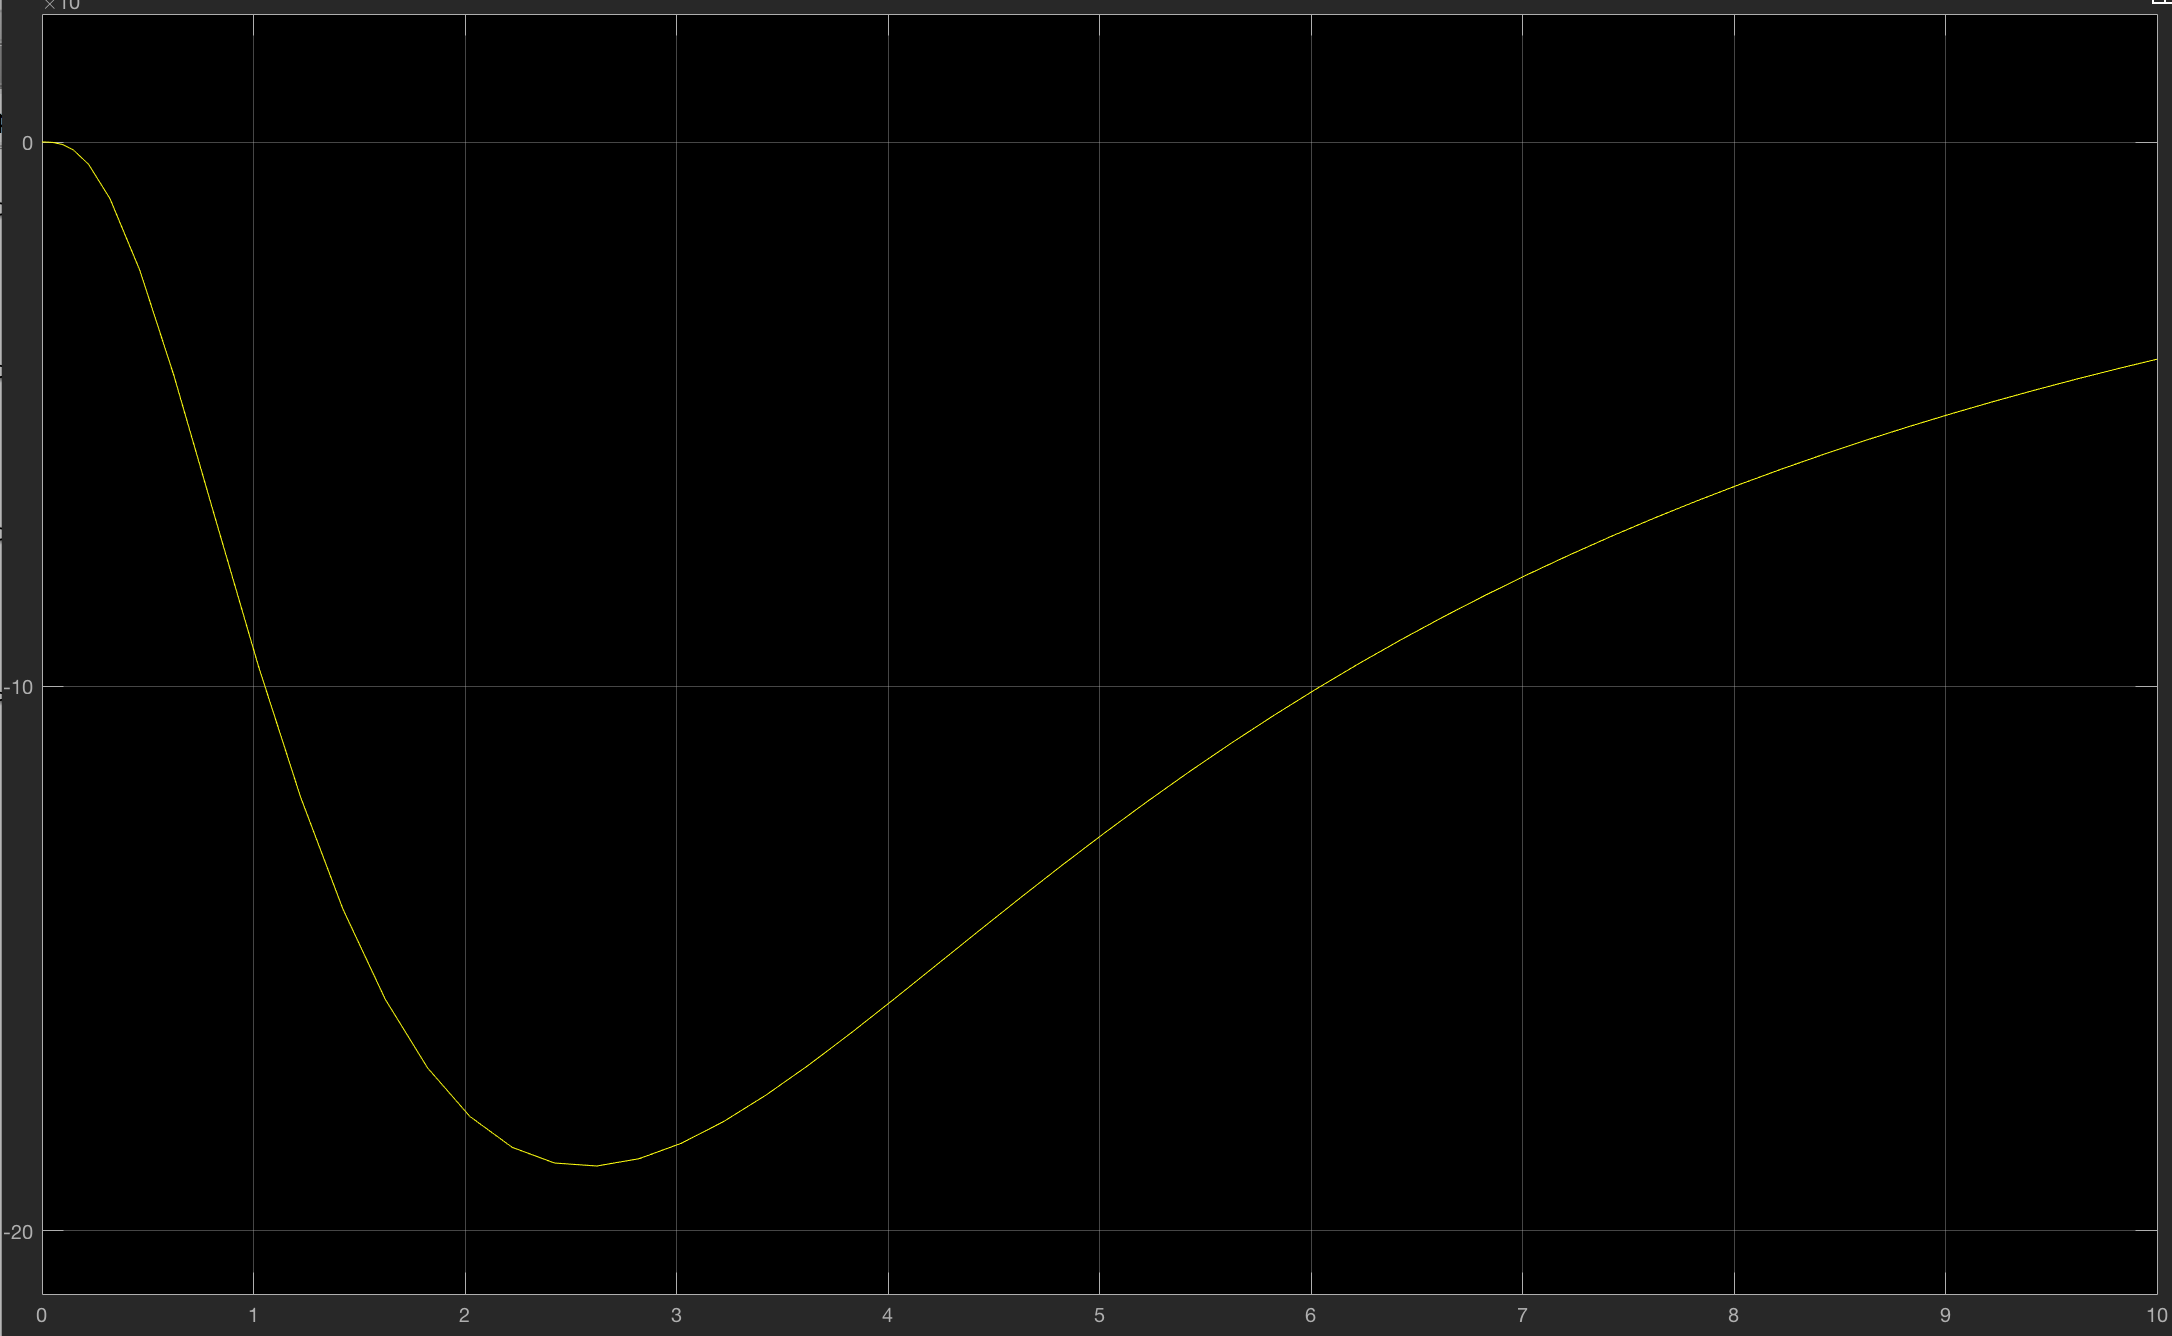
\includegraphics[width=1\textwidth]{images/closedloopGzstep.png}
	\caption{smth.}
	\label{closedloop4}
\end{figure}

\begin{figure}[H]
  \centering
    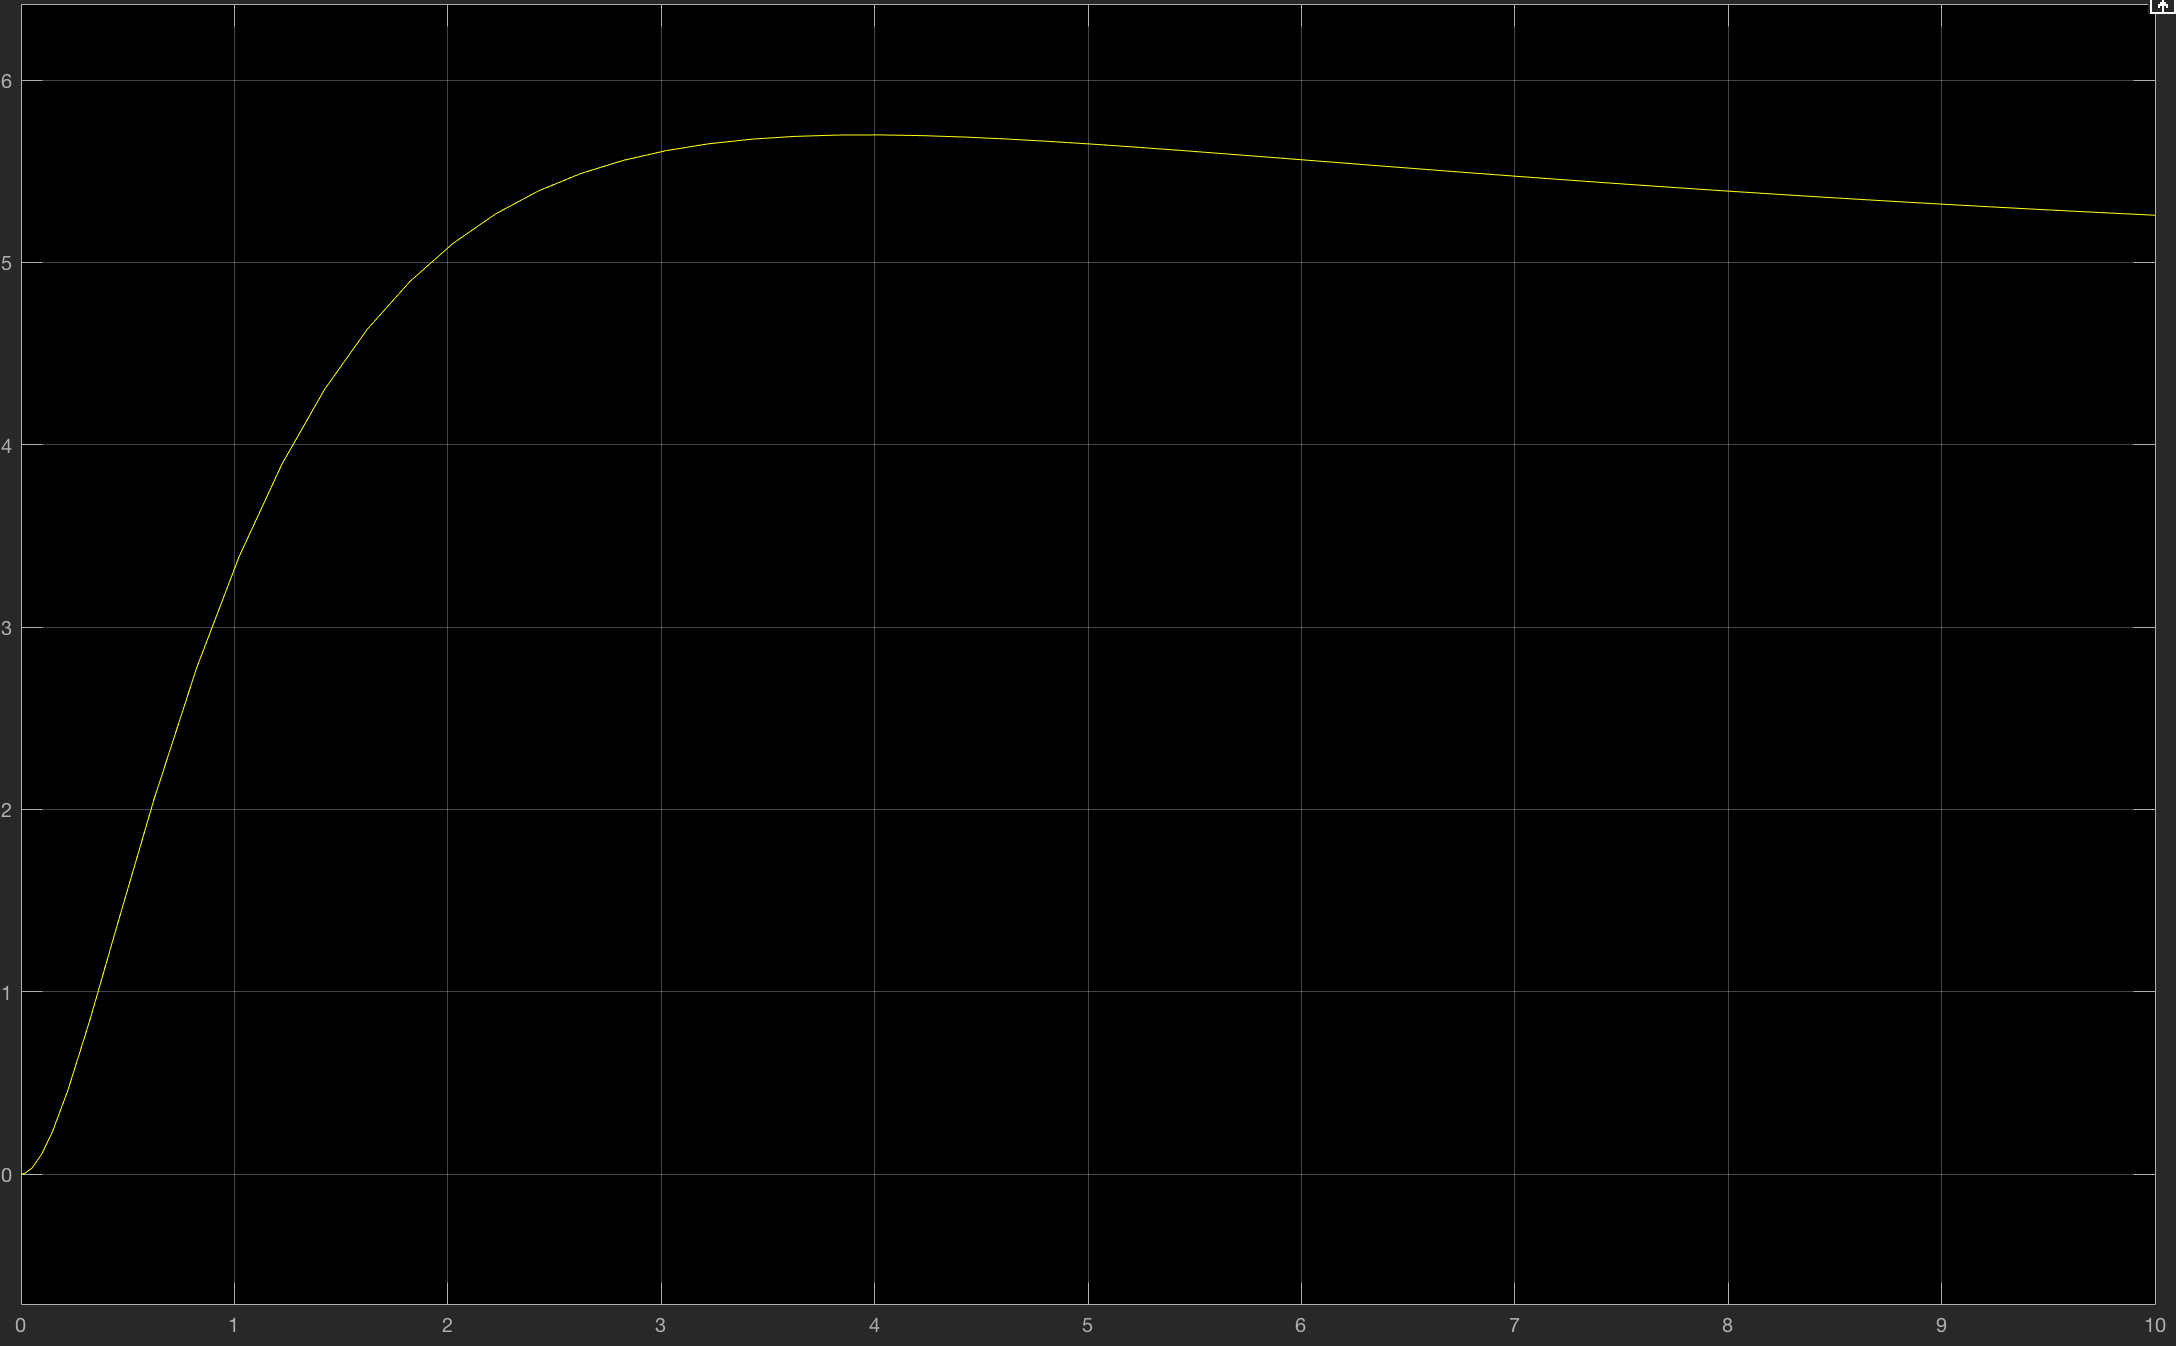
\includegraphics[width=1\textwidth]{images/closedloopNystep.png}
	\caption{smth.}
	\label{closedloop5}
\end{figure}

